\documentclass[11pt,a4paper]{article}
\usepackage[margin=2.3cm]{geometry}
\usepackage{amsmath,amssymb,bm}
\usepackage{graphicx}
\usepackage{booktabs}
\usepackage{natbib}
\usepackage[colorlinks=true,linkcolor=blue,citecolor=blue,urlcolor=blue]{hyperref}
\usepackage{xcolor}

\graphicspath{{../../figures/}}

\newcommand{\feh}{\ensuremath{[\mathrm{Fe/H}]}}
\newcommand{\sig}{\ensuremath{\sigma}}
\newcommand{\N}{\ensuremath{\mathcal{N}}}

\title{Deconvolving the age--metallicity distribution of APOGEE DR17 giants:\\
the current extreme-deconvolution model, its failure mode,\\ and a proposal for a calibrated model}
\author{Eos project working note}
\date{25 September 2026}

\begin{document}
\maketitle

\section*{Summary}
\begin{itemize}
  \item We fit the joint distribution of AstroNN age and APOGEE \feh{} for 164{,}215 giants with extreme deconvolution \citep[XD;][]{Bovy2011}: a Gaussian mixture convolved with each star's measurement covariance, with the number of components $K$ chosen by five-fold held-out log density.
  \item The fitted \emph{deconvolved} density is made of needle-like components: 17 of 20 components at $K=20$ have intrinsic age widths below $0.45$\,Gyr, while the median quoted age error is $1.29$\,Gyr.
  \item Cause: the XD noise model, $\hat a = a + \epsilon$, is contradicted by the data. For high-$\alpha$ stars, the observed age scatter is \emph{smaller} than the quoted total age error in every \feh{} bin (0.9--1.4\,Gyr vs 1.6--3.2\,Gyr). This is the signature of a shrinkage estimator, not additive noise. XD can satisfy it only by sending intrinsic age variances towards zero.
  \item Held-out likelihood cannot detect this. It scores the noise-convolved model, which is insensitive to intrinsic structure below the noise scale.
  \item Proposal: fit in $(\ln a, \feh)$; replace the quoted AstroNN errors with a \emph{calibrated linear-Gaussian measurement model} $\hat{\bm y} = \mathbf{R}\bm v + \bm c + \bm\epsilon$, derived from asteroseismic ages \citep[APOKASC-3;][]{Pinsonneault2025}. XD handles this exactly through its projection matrices. Add bounded support, a covariance prior, paired cross-validation, and injection--recovery validation.
\end{itemize}

\section{Data and sample}
\label{sec:data}
The sample is the base selection of the Eos figures repository (\texttt{eos\_figures/data.py}): APOGEE DR17 \texttt{allStarLite} \citep{DR17} matched to the AstroNN DR17 value-added catalogue \citep{Leung2019,Mackereth2019}. It is restricted to red giants ($\log g<3$) with velocity errors $<50$\,km\,s$^{-1}$, abundance errors $<0.2$\,dex, heliocentric distance $<15$\,kpc, no Magellanic Cloud targets, and no stars near known satellites or in the Vasiliev globular-cluster member list. This leaves 210{,}392 stars.

The \emph{good-age} subsample (mask \texttt{base\_age}) further requires a finite, positive AstroNN age and $\sigma_{\rm model}/a<0.2$, where $\sigma_{\rm model}$ is \texttt{age\_model\_error}. It contains 164{,}215 stars. Figure~\ref{fig:data} shows its density in the age--\feh{} plane.

The deconvolution uses two error columns:
\begin{itemize}
  \item \texttt{age\_total\_error} ($\sigma_{\rm tot}$), AstroNN's combined model and propagated-measurement uncertainty. Among good-age stars, $\sigma_{\rm tot}/\sigma_{\rm model}$ has 1st, 16th, 50th, 84th and 99th percentiles of 1.01, 1.12, 1.63, 2.45 and 4.58.
  \item \texttt{fe\_h\_err}, APOGEE's \feh{} error, with median $0.009$\,dex.
\end{itemize}
In practice the \feh{} dimension is noiseless compared with the age dimension.

\begin{figure}[t]
  \centering
  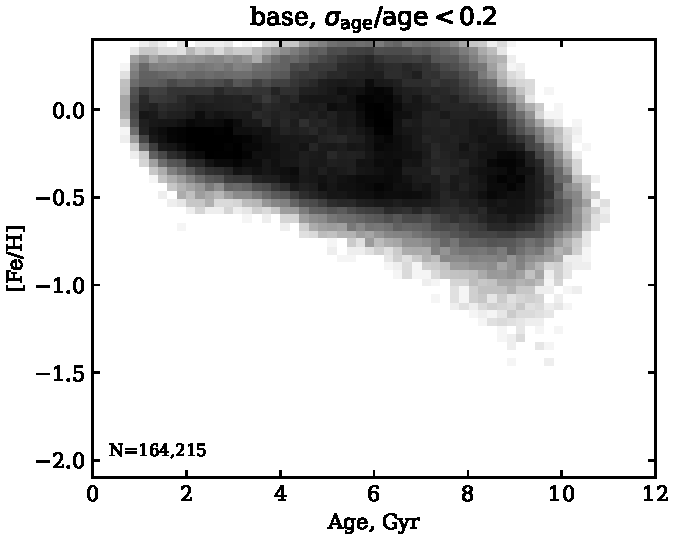
\includegraphics[width=0.55\textwidth]{eos_age_feh_density.pdf}
  \caption{Observed density of the 164{,}215 good-age stars: $\log_{10}$ counts in $0.2\,{\rm Gyr}\times0.045$\,dex bins, grey stretch between the 10th and 99th percentiles.}
  \label{fig:data}
\end{figure}

\section{The current model}
\label{sec:current}

\subsection{Extreme deconvolution}
Let $\bm v_i=(a_i,\feh_i)$ be the true age and metallicity of star $i$, $\bm w_i$ the measured values, and $\mathbf S_i$ the measurement covariance. XD assumes
\begin{equation}
  \bm w_i = \bm v_i + \bm\epsilon_i,\qquad \bm\epsilon_i\sim\N(\bm 0,\mathbf S_i),\qquad
  p(\bm v)=\sum_{k=1}^{K}\alpha_k\,\N(\bm v\mid\bm\mu_k,\mathbf V_k),
  \label{eq:xd_model}
\end{equation}
so that the likelihood of the data is
\begin{equation}
  \ln\mathcal L=\sum_i\ln\sum_k\alpha_k\,\N(\bm w_i\mid\bm\mu_k,\mathbf T_{ik}),\qquad \mathbf T_{ik}=\mathbf V_k+\mathbf S_i .
  \label{eq:xd_like}
\end{equation}
The EM iteration of \citet{Bovy2011} alternates two steps. The E step computes the responsibilities $q_{ik}\propto\alpha_k\N(\bm w_i\mid\bm\mu_k,\mathbf T_{ik})$ and the conditional moments
\begin{align}
  \bm b_{ik}&=\bm\mu_k+\mathbf V_k\mathbf T_{ik}^{-1}(\bm w_i-\bm\mu_k), &
  \mathbf B_{ik}&=\mathbf V_k-\mathbf V_k\mathbf T_{ik}^{-1}\mathbf V_k .
\end{align}
The M step updates
\begin{equation}
  \alpha_k=\frac{1}{n}\sum_i q_{ik},\qquad
  \bm\mu_k=\frac{\sum_i q_{ik}\bm b_{ik}}{\sum_i q_{ik}},\qquad
  \mathbf V_k=\frac{\sum_i q_{ik}\left[(\bm\mu_k-\bm b_{ik})(\bm\mu_k-\bm b_{ik})^{\!\top}+\mathbf B_{ik}\right]}{\sum_i q_{ik}} .
\end{equation}

\subsection{Implementation}
The code, \texttt{eos\_figures/xd.py}, is a port of the numpy XD in the \texttt{qso\_p\_color} project, restricted to fully observed data:
\begin{itemize}
  \item \textbf{2D fast path.} A closed-form element-wise $2\times2$ E/M step matches the generic batched algebra to $2\times10^{-13}$, and \texttt{log\_gauss} matches \texttt{scipy} to $2\times10^{-14}$. At $K=8$, $n=164{,}215$ it reduces the time per iteration from $0.64$\,s to $0.076$\,s.
  \item \textbf{Numerical care.} Second moments are accumulated about the previous mean, and the reported likelihood is recomputed for the returned mixture.
  \item \textbf{Noise model.} $\mathbf S_i=\mathrm{diag}(\sigma_{{\rm tot},i}^2,\ \sigma_{\feh,i}^2)$, with no age--\feh{} error covariance.
  \item \textbf{Convergence.} At $K=8$ with no tolerance, the mean log-likelihood per star still rose by $2.2\times10^{-3}$ after iteration 2000, alternating plateaus and jumps. A single-step tolerance therefore stops too early. We stop when the mean per-star gain, averaged over the last 50 iterations, falls below $3\times10^{-7}|\ln\mathcal L/n|$ (about 0.1 in total $\ln\mathcal L$ per iteration), with at most 3000 iterations.
  \item \textbf{Initialisation.} At $K=8$ we tested three seeds each. $k$-means++ starts converge in about 730 iterations but reach $\ln\mathcal L/n=-2.2475$. Random-row starts (the \texttt{qso\_p\_color} default) take 1200--1500 iterations but reach $-2.2447$, better by $2.8\times10^{-3}$ per star ($\approx460$ in total). Random starts are used.
  \item \textbf{Tests.} Nine tests: \texttt{tests/test\_xd.py} (recovering intrinsic widths; two-component recovery; heteroscedastic anisotropic noise; monotone likelihood; CV complexity choice; BIC penalty) and \texttt{tests/test\_xd\_age\_feh.py} (grid counts integrate to $N$; the error-grouping approximation matches the exact per-star sum to $<1\%$ of the peak; convolved counts match a $2\times10^5$-star Monte Carlo, with pull mean $<0.3$ and pull width in 0.7--1.3).
\end{itemize}

\subsection{Model selection}
Following \texttt{qso\_p\_color}, $K$ is chosen to maximise the five-fold held-out log density of the \emph{observed} data under the convolved model, eq.~\eqref{eq:xd_like}. Each (K, fold) pair uses two random restarts, and the restart with the higher \emph{training} likelihood is kept, so model choice never sees the validation data.

BIC and AIC are computed from full-sample fits for comparison. They are not used for the decision, because mixtures are singular models and the regularity conditions behind BIC fail.

The runner, \texttt{scripts/fit\_xd\_age\_feh.py}, is parallel and resumable, writing one JSON file per job.

Table~\ref{tab:cv} gives the held-out scores for the values of $K$ completed so far. They rise steeply up to $K\approx12$ and flatten beyond $K\approx16$. The quoted standard error ($1.76\times10^{-3}$) is that of each $K$'s mean on its own; it is dominated by star-to-star scatter shared by all $K$. Differences between $K$ need \emph{paired} per-star comparisons, which the proposed model stores (Sec.~\ref{sec:selection}).

\begin{table}[t]
  \centering
  \caption{Five-fold held-out mean log density per star (natural log; units of $\ln[{\rm Gyr}^{-1}{\rm dex}^{-1}]$) for the current model. $\Delta$ is relative to the best completed $K$. All folds converged. $K\le7$ was still running when this note was written.}
  \label{tab:cv}
  \begin{tabular}{rrr@{\hspace{2em}}rrr}
    \toprule
    $K$ & CV & $\Delta$ & $K$ & CV & $\Delta$\\
    \midrule
     8 & $-2.24596$ & $-0.00557$ & 15 & $-2.24102$ & $-0.00063$\\
     9 & $-2.24347$ & $-0.00308$ & 16 & $-2.24059$ & $-0.00020$\\
    10 & $-2.24213$ & $-0.00174$ & 17 & $-2.24051$ & $-0.00012$\\
    11 & $-2.24160$ & $-0.00121$ & 18 & $-2.24069$ & $-0.00030$\\
    12 & $-2.24123$ & $-0.00084$ & 19 & $-2.24066$ & $-0.00027$\\
    13 & $-2.24110$ & $-0.00071$ & 20 & $-2.24039$ & $0$\\
    14 & $-2.24089$ & $-0.00050$ &    &            &          \\
    \bottomrule
  \end{tabular}
\end{table}

\subsection{Evaluating the model on the plotting grid}
The \emph{deconvolved} model gives expected counts $n\int_{\rm bin}p(\bm v)\,d\bm v$, integrated by the midpoint rule on $5\times5$ sub-cells per bin. The \emph{convolved} model gives $\sum_i\int_{\rm bin}\sum_k\alpha_k\N(\bm x\mid\bm\mu_k,\mathbf V_k+\mathbf S_i)\,d\bm x$. For speed, stars are grouped on a $40\times40$ grid in $(\ln\sigma_a,\ln\sigma_{\feh})$, and each group uses its mean variances; the tests above bound the resulting error. Both are implemented in \texttt{eos\_figures/xd\_age\_feh.py}.

\subsection{Result: a needle-like deconvolved density}
Figure~\ref{fig:k20} shows the deconvolved density of the best available $K=20$ model. This is fold model \texttt{K20\_f4\_r0}, trained on 80\% of the stars; it scores highest of the ten $K=20$ fold models when evaluated on all stars ($\ln\mathcal L/n=-2.23991$). Table~\ref{tab:k20} lists its components:
\begin{itemize}
  \item 17 of the 20 components have $\sigma_a<0.45$\,Gyr, and several are almost degenerate lines ($|\rho|$ up to 0.99).
  \item The three heaviest components near $a\approx8.1$\,Gyr carry 28\% of the weight, with $\sigma_a=0.11$--$0.24$\,Gyr.
\end{itemize}
These widths are far below anything the data could resolve, given $\sigma_{\rm tot}\sim1$--3\,Gyr.

\begin{figure}[t]
  \centering
  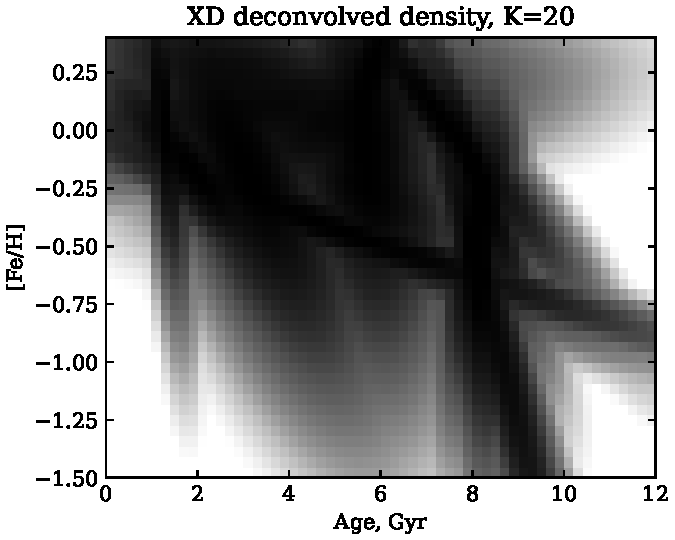
\includegraphics[width=0.55\textwidth]{eos_age_feh_xd_deconvolved.pdf}
  \caption{Deconvolved density of the current model (preliminary $K=20$ fold model), shown as expected counts per bin on the grid of Fig.~\ref{fig:data}.}
  \label{fig:k20}
\end{figure}

\begin{table}[t]
  \centering
  \small
  \caption{Components of the $K=20$ model of Fig.~\ref{fig:k20}, sorted by weight. $\sigma_a$ and $\sigma_{\rm Fe}$ are intrinsic widths (Gyr, dex); $\rho$ is the age--\feh{} correlation.}
  \label{tab:k20}
  \begin{tabular}{rrrrrr}
    \toprule
    $\alpha_k$ & $\mu_a$ [Gyr] & $\mu_{\rm Fe}$ & $\sigma_a$ [Gyr] & $\sigma_{\rm Fe}$ & $\rho$\\
    \midrule
0.142 & 2.92 & $-0.12$ & 0.392 & 0.160 & $-0.67$ \\
0.114 & 8.17 & $-0.40$ & 0.110 & 0.107 & $+0.74$ \\
0.095 & 5.20 & $-0.44$ & 1.221 & 0.088 & $-0.99$ \\
0.092 & 8.09 & $-0.60$ & 0.138 & 0.109 & $-0.83$ \\
0.079 & 8.00 & $-0.16$ & 0.238 & 0.116 & $-0.95$ \\
0.065 & 5.53 & $+0.00$ & 0.254 & 0.094 & $-0.31$ \\
0.060 & 5.77 & $+0.26$ & 0.190 & 0.087 & $+0.82$ \\
0.056 & 1.84 & $-0.17$ & 0.337 & 0.083 & $-0.87$ \\
0.048 & 5.77 & $-0.28$ & 0.227 & 0.079 & $+0.75$ \\
0.035 & 3.43 & $-0.24$ & 0.244 & 0.088 & $-0.06$ \\
0.031 & 1.27 & $+0.05$ & 0.060 & 0.116 & $-0.68$ \\
0.031 & 7.29 & $+0.03$ & 0.399 & 0.080 & $-0.88$ \\
0.027 & 6.61 & $+0.18$ & 0.442 & 0.078 & $-0.84$ \\
0.025 & 4.16 & $+0.08$ & 1.039 & 0.052 & $+0.15$ \\
0.025 & 5.65 & $-0.11$ & 0.224 & 0.118 & $-0.34$ \\
0.020 & 5.59 & $-0.10$ & 0.267 & 0.120 & $-0.23$ \\
0.018 & 8.33 & $-0.71$ & 0.303 & 0.292 & $-0.97$ \\
0.018 & 5.65 & $-0.14$ & 0.241 & 0.108 & $-0.12$ \\
0.014 & 4.02 & $+0.17$ & 0.949 & 0.081 & $-0.84$ \\
0.004 & 8.67 & $-0.86$ & 0.273 & 0.077 & $-0.93$ \\
    \bottomrule
  \end{tabular}
\end{table}

\section{Why a better model is needed}
\label{sec:motivation}

\subsection{What the intrinsic density should look like}
\label{sec:expect}
Established Milky Way structure suggests three components with distinct shapes in the age--\feh{} plane:
\begin{enumerate}
  \item \textbf{Low-$\alpha$ (thin) disc:} ages $\sim0$--8\,Gyr and $-0.7\lesssim\feh\lesssim+0.4$. The mean age--metallicity relation is nearly flat, with a large spread in \feh{} at fixed age ($\sim0.2$\,dex, in part from radial migration). The density should be broad and smooth on scales $\gtrsim1$\,Gyr, apart from possible modest star-formation bursts.
  \item \textbf{High-$\alpha$ (thick) disc:} ages $\sim8$--12\,Gyr, following a tight, tilted age--metallicity sequence in which \feh{} rises from $\sim-1$ to $\sim0$ as age decreases \citep{Haywood2013}. A narrow, negatively correlated ridge is physical here.
  \item \textbf{Old metal-poor populations:} the accreted GS/E debris \citep{Belokurov2018,Helmi2018} and the in-situ \textit{Aurora} population \citep{Belokurov2022}, at ages $\gtrsim10$\,Gyr and $\feh\lesssim-0.7$.
\end{enumerate}
The support is bounded: $0<a\lesssim13.8$\,Gyr. The density also includes the selection function: APOGEE targeting, and the number of giants per unit stellar mass formed, which depends on age. It is not the star-formation history.

\subsection{The additive-noise model is contradicted by the data}
\label{sec:test}
If $\hat a=a+\epsilon$ with $\epsilon$ independent of $a$ and ${\rm Var}(\epsilon)=\sigma^2$, then within any subsample
\begin{equation}
  {\rm Var}(\hat a)={\rm Var}(a)+\langle\sigma^2\rangle\ \ge\ \langle\sigma^2\rangle .
  \label{eq:additive}
\end{equation}
Figure~\ref{fig:consistency} tests this in 0.1-dex \feh{} bins; Table~\ref{tab:consistency} gives 0.2-dex values:
\begin{itemize}
  \item For high-$\alpha$ stars the inequality fails with $\sigma_{\rm tot}$ in \emph{every} bin: ${\rm std}(\hat a)=0.9$--1.4\,Gyr against rms $\sigma_{\rm tot}=1.6$--3.2\,Gyr.
  \item For all good-age stars it holds only for $-0.4<\feh<+0.2$.
  \item Even the smaller $\sigma_{\rm model}$ violates it for $\feh<-0.8$ (all good-age stars) and $\feh<-0.6$ (high-$\alpha$).
\end{itemize}
Under eq.~\eqref{eq:xd_model}, the maximum-likelihood response to $\langle\sigma^2\rangle>{\rm Var}(\hat a)$ is $\mathbf V_k^{aa}\to0$: exactly the needles of Fig.~\ref{fig:k20}.

\begin{figure}[t]
  \centering
  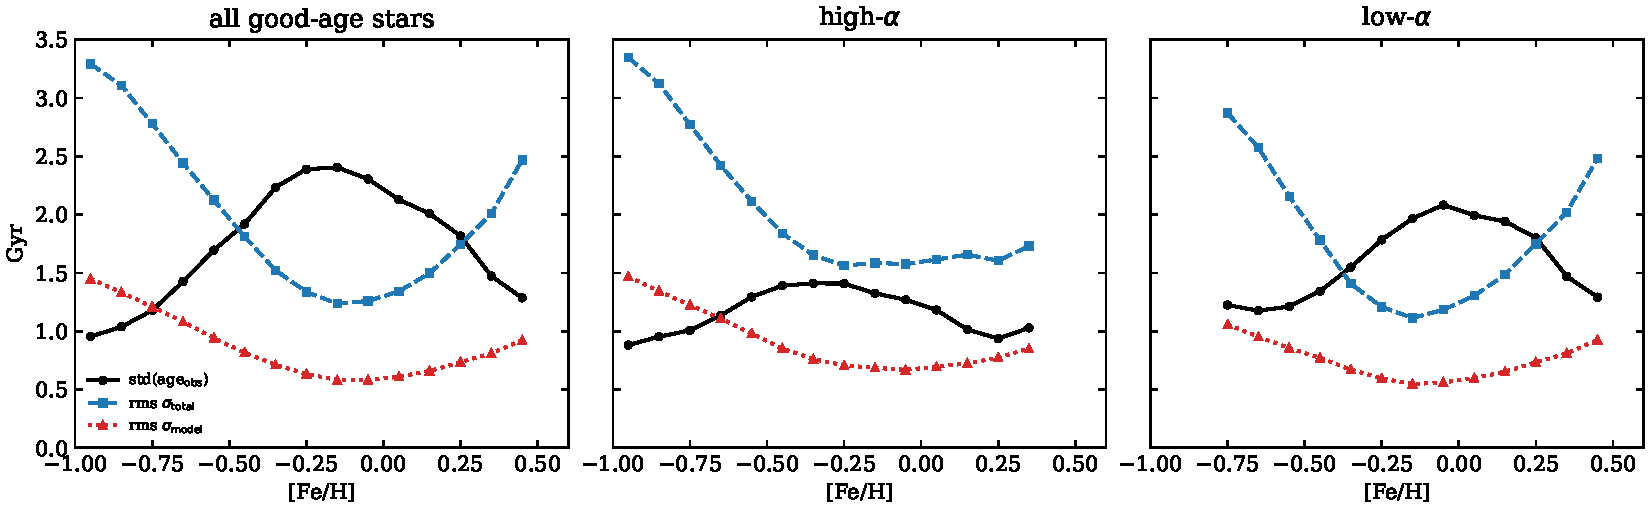
\includegraphics[width=\textwidth]{eos_age_err_consistency.pdf}
  \caption{Observed age scatter (black) compared with the rms quoted total (blue) and model (red) AstroNN age errors, in 0.1-dex \feh{} bins. Additive noise requires the black curve to lie above the error curves.}
  \label{fig:consistency}
\end{figure}

\begin{table}[t]
  \centering
  \small
  \caption{Additive-noise test, eq.~\eqref{eq:additive}, in 0.2-dex bins: ${\rm Var}(\hat a)-\langle\sigma^2\rangle$ in Gyr$^2$. Negative entries are inconsistent with additive noise.}
  \label{tab:consistency}
  \begin{tabular}{lrrrr}
    \toprule
    & \multicolumn{2}{c}{all good-age} & \multicolumn{2}{c}{high-$\alpha$}\\
    \feh{} bin & $\sigma_{\rm tot}$ & $\sigma_{\rm model}$ & $\sigma_{\rm tot}$ & $\sigma_{\rm model}$\\
    \midrule
    $-1.0$ to $-0.8$ & $-8.99$ & $-0.85$ & $-9.29$ & $-1.03$\\
    $-0.8$ to $-0.6$ & $-4.66$ & $+0.59$ & $-5.26$ & $-0.12$\\
    $-0.6$ to $-0.4$ & $-0.31$ & $+2.71$ & $-2.06$ & $+0.99$\\
    $-0.4$ to $-0.2$ & $+3.45$ & $+5.04$ & $-0.61$ & $+1.45$\\
    $-0.2$ to $\phantom{+}0.0$ & $+4.00$ & $+5.22$ & $-0.80$ & $+1.24$\\
    $\phantom{+}0.0$ to $+0.2$ & $+2.35$ & $+3.93$ & $-1.38$ & $+0.78$\\
    $+0.2$ to $+0.4$ & $-0.36$ & $+2.41$ & $-1.73$ & $+0.33$\\
    \bottomrule
  \end{tabular}
\end{table}

\subsection{Interpretation: AstroNN ages behave like shrinkage estimates}
A regression network trained on asteroseismic ages \citep[APOKASC-2;][]{Pinsonneault2018} returns something closer to a posterior mean, $\hat a\approx{\rm E}[a\mid{\rm spectrum}]$, than to a noisy copy of $a$. By the law of total variance,
\begin{equation}
  {\rm Var}(\hat a)={\rm Var}(a)-{\rm E}\!\left[{\rm Var}(a\mid{\rm spectrum})\right],
\end{equation}
so the estimates are \emph{under}-dispersed, and the quoted uncertainty measures posterior width, not scatter about the truth.

For a Gaussian prior (the training-set distribution) $\N(m_0,P)$ and a Gaussian likelihood of width $s$, the posterior mean is $\hat a=(1-\lambda)a+\lambda m_0+\eta$ with $\lambda=s^2/(s^2+P)$. This is a linear map with slope $\beta=1-\lambda<1$, plus noise.

Two further observations point the same way:
\begin{itemize}
  \item \textbf{A ceiling.} Only 0.65\% of good-age stars have $\hat a>10$\,Gyr and 0.02\% have $\hat a>11$\,Gyr, with a maximum of 12.25\,Gyr. This conflicts with the expected 10--13\,Gyr high-$\alpha$ and halo populations (Sec.~\ref{sec:expect}).
  \item \textbf{The largest errors fall where the training data are sparse.} The median $\sigma_{\rm tot}$ exceeds 2--3\,Gyr at $\feh<-0.6$ and 7--11\,Gyr (Fig.~\ref{fig:errdist}).
\end{itemize}

\begin{figure}[t]
  \centering
  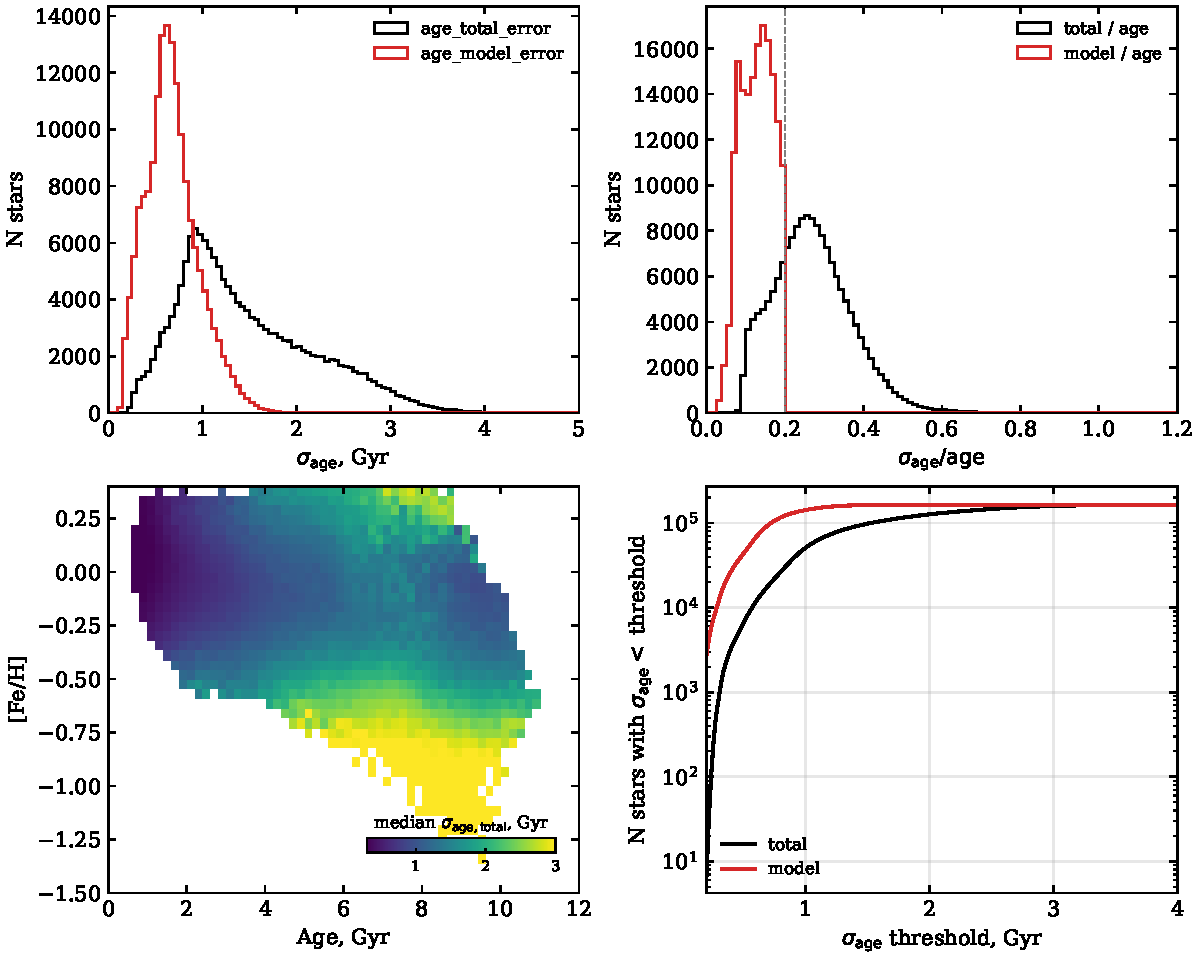
\includegraphics[width=0.8\textwidth]{eos_age_err_dist.pdf}
  \caption{AstroNN age errors of the good-age sample:
  \emph{top left}, distributions of $\sigma_{\rm tot}$ and $\sigma_{\rm model}$;
  \emph{top right}, fractional errors, with the dashed line marking the $\sigma_{\rm model}/a<0.2$ selection;
  \emph{bottom left}, median $\sigma_{\rm tot}$ across the age--\feh{} plane;
  \emph{bottom right}, the number of stars below an error threshold.}
  \label{fig:errdist}
\end{figure}

\subsection{Further limitations of the current set-up}
\begin{itemize}
  \item \textbf{Linear age.} Errors are close to fractional (median $\sigma_{\rm tot}/\hat a=0.31, 0.28, 0.27, 0.26, 0.19, 0.18$ for 0--2, 2--4, 4--6, 6--8, 8--10 and 10--13\,Gyr), so they are closer to Gaussian in $\ln a$. Gaussian components in linear $a$ also put probability at $a<0$ and above the age of the Universe.
  \item \textbf{Weak identifiability.} Held-out likelihood evaluates $\mathbf V_k+\mathbf S_i$. When $\mathbf S_i\gg\mathbf V_k$, very different intrinsic densities give almost the same score, so CV chooses $K$ but cannot regularise intrinsic widths.
  \item \textbf{Selection on error.} Cutting on $\sigma$ does not help. Stars with $\sigma_{\rm tot}<1$\,Gyr include none with $\feh<-0.5$, and $\sigma_{\rm tot}<2.5$\,Gyr keeps only 61\% of $\feh<-0.5$ stars against 89\% overall. The cut is a value-dependent selection that XD does not model.
  \item \textbf{Unpaired standard errors} in Table~\ref{tab:cv} overstate the uncertainty on differences between $K$ values.
\end{itemize}

\section{Proposed model}
\label{sec:proposal}

\subsection{Variables}
Fit $\bm v=(\ell,\feh)$ with $\ell=\ln(a/{\rm Gyr})$. The data are $\hat{\bm y}_i=(\ln\hat a_i,\ \widehat{\feh}_i)$.

\subsection{Calibrated measurement model}
Replace eq.~\eqref{eq:xd_model} by a linear-Gaussian measurement model,
\begin{equation}
  \hat{\bm y}_i=\mathbf R_i\,\bm v_i+\bm c_i+\bm\epsilon_i,\qquad
  \mathbf R_i=\begin{pmatrix}\beta(\bm z_i)&0\\0&1\end{pmatrix},\quad
  \bm c_i=\begin{pmatrix}\gamma(\bm z_i)\\0\end{pmatrix},\quad
  \bm\epsilon_i\sim\N\!\left(\bm 0,\ \mathrm{diag}\!\left[\tau^2(\bm z_i),\ \sigma^2_{\feh,i}\right]\right).
  \label{eq:meas}
\end{equation}
Here $\bm z_i$ are observables on which the calibration may depend: \feh, [$\alpha$/Fe], $\log g$, S/N, or the quoted $\sigma_{\rm model}$.

The functions $\beta$ (slope; $\beta<1$ is shrinkage), $\gamma$ (offset) and $\tau$ (true residual scatter) are \emph{fitted} on stars with asteroseismic ages. We would use the APOKASC-3 catalogue \citep{Pinsonneault2025}, restricted to stars not used to train AstroNN or held out from its training. The calibration regression is itself an errors-in-variables fit, since asteroseismic ages have their own uncertainties. It is low-dimensional and can be done by maximum likelihood, e.g.\ piecewise-linear $\beta,\gamma,\tau$ in \feh{} and [$\alpha$/Fe].

\textbf{Checks on the calibration.}
\begin{itemize}
  \item The additive test of Sec.~\ref{sec:test} generalises to ${\rm Var}(\hat\ell)=\beta^2{\rm Var}(\ell)+\langle\tau^2\rangle$, which must hold in every bin.
  \item The calibration sample's coverage in \feh{} and age must be reported. Outside it, the model extrapolates, and the fitted density must be flagged there.
\end{itemize}

\subsection{XD with projection}
Equation~\eqref{eq:meas} is exactly the form handled by XD through per-object projection matrices \citep[][their Sec.~2]{Bovy2011}:
\begin{align}
  \mathbf T_{ik}&=\mathbf R_i\mathbf V_k\mathbf R_i^{\top}+\mathbf S_i,\\
  \bm b_{ik}&=\bm\mu_k+\mathbf V_k\mathbf R_i^{\top}\mathbf T_{ik}^{-1}\left(\hat{\bm y}_i-\mathbf R_i\bm\mu_k-\bm c_i\right),\\
  \mathbf B_{ik}&=\mathbf V_k-\mathbf V_k\mathbf R_i^{\top}\mathbf T_{ik}^{-1}\mathbf R_i\mathbf V_k,
\end{align}
with the M step unchanged. With $\beta<1$, the intrinsic spread needed to explain a given observed spread \emph{increases}, removing the pressure towards $\mathbf V_k^{\ell\ell}\to0$.

The change to \texttt{eos\_figures/xd.py} is small: $\mathbf R_i$ is diagonal and $2\times2$, so the element-wise fast path extends directly.

\subsection{Bounded support}
Truncate the mixture at $\ell_{\max}=\ln13.8$. The likelihood of star $i$ becomes $\int_{\ell<\ell_{\max}}\N(\hat{\bm y}_i\mid\mathbf R_i\bm v+\bm c_i,\mathbf S_i)\,p(\bm v)\,d\bm v/Z$, where $Z=\sum_k\alpha_k\Phi_k$ and $\Phi_k$ is the mass of component $k$ below $\ell_{\max}$. For Gaussian components this needs only univariate normal CDFs.

As a cheaper first step: fit without truncation, report the leaked mass $1-Z$, and implement truncation only if the leakage exceeds 1\%.

\subsection{Covariance prior}
Use MAP-EM with an inverse-Wishart prior on each $\mathbf V_k$, so that the M step becomes $\mathbf V_k=(\sum_i q_{ik}[\ldots]+\bm\Psi)/(\sum_i q_{ik}+\nu+3)$. Bovy et al.'s regularisation parameter $w$ corresponds to $\bm\Psi=w\mathbf I$.

The floor should be tied to what the calibrated data can resolve: $\Psi^{\ell\ell}\sim(0.05)^2$ (a 5\% age width) and $\Psi^{\rm FeFe}\sim(0.02\,{\rm dex})^2$. The results must be shown to be stable when these values are halved and doubled.

\subsection{Model selection and posterior-predictive checks}
\label{sec:selection}
\begin{itemize}
  \item \textbf{Choosing $K$.} Five-fold held-out log density as now, but storing per-star held-out $\ln p$ so that differences between $K$ values carry \emph{paired} standard errors. Choose the smallest $K$ within one paired standard error of the maximum.
  \item \textbf{Checks.}
  \begin{enumerate}
    \item data $-$ convolved-model residual maps, with the $\chi^2$ per bin;
    \item the calibrated variance test above, applied to model draws;
    \item marginal age distributions for the high-$\alpha$, low-$\alpha$ and metal-poor subsets, data against model.
  \end{enumerate}
\end{itemize}

\subsection{Validation by injection--recovery}
Build a mock intrinsic density with the three components of Sec.~\ref{sec:expect}:
\begin{itemize}
  \item a broad thin disc;
  \item a tilted, narrow thick-disc sequence;
  \item an old metal-poor tail up to 13\,Gyr.
\end{itemize}
Draw 164{,}215 stars, map them through eq.~\eqref{eq:meas} with the calibrated $\beta,\gamma,\tau$, fit, and compare the recovered deconvolved density with the truth. Metrics: the mean and width of $\ell$ at fixed \feh{}, component weights, and the Kullback--Leibler divergence on the grid.

Run the same mock through the \emph{current} model (additive noise with $\sigma_{\rm tot}$) to show that it produces needle artefacts. This makes the failure mode demonstrable rather than inferred.

\subsection{Cost}
The current runner does 200 CV fits at $K\le20$ in $\sim$2 hours on 12 cores when the machine is not oversubscribed. With a calibrated model, $K$ is expected to be well below 20. With early stopping on the held-out score as $K$ increases, CV should need well under an hour.

\section{Next steps}
\begin{enumerate}
  \item Stop the current CV run, which uses a contradicted noise model, or keep it only as the ``current model'' baseline for the injection--recovery comparison.
  \item Cross-match the sample with APOKASC-3; fit $\beta,\gamma,\tau$ and repeat the variance test with the calibrated model.
  \item Implement projection XD in $(\ln a,\feh)$ with an inverse-Wishart prior and paired CV; run injection--recovery; then refit the data and make the four-panel figure (data, deconvolved, convolved, residual).
\end{enumerate}

\begin{thebibliography}{99}
\bibitem[Abdurro'uf et al.(2022)]{DR17} Abdurro'uf et al., 2022, ApJS, 259, 35, \emph{The Seventeenth Data Release of the Sloan Digital Sky Surveys}. \href{https://doi.org/10.3847/1538-4365/ac4414}{doi:10.3847/1538-4365/ac4414}, \href{https://arxiv.org/abs/2112.02026}{arXiv:2112.02026}.
\bibitem[Belokurov et al.(2018)]{Belokurov2018} Belokurov V., Erkal D., Evans N.~W., Koposov S.~E., Deason A.~J., 2018, MNRAS, 478, 611, \emph{Co-formation of the disc and the stellar halo}. \href{https://doi.org/10.1093/mnras/sty982}{doi:10.1093/mnras/sty982}, \href{https://arxiv.org/abs/1802.03414}{arXiv:1802.03414}.
\bibitem[Belokurov \& Kravtsov(2022)]{Belokurov2022} Belokurov V., Kravtsov A., 2022, MNRAS, 514, 689, \emph{From dawn till disc: Milky Way's turbulent youth revealed by the APOGEE+Gaia data}. \href{https://doi.org/10.1093/mnras/stac1267}{doi:10.1093/mnras/stac1267}, \href{https://arxiv.org/abs/2203.04980}{arXiv:2203.04980}.
\bibitem[Bovy et al.(2011)]{Bovy2011} Bovy J., Hogg D.~W., Roweis S.~T., 2011, Ann. Appl. Stat., 5, 1657, \emph{Extreme deconvolution: inferring complete distribution functions from noisy, heterogeneous and incomplete observations}. \href{https://doi.org/10.1214/10-AOAS439}{doi:10.1214/10-AOAS439}, \href{https://arxiv.org/abs/0905.2979}{arXiv:0905.2979}.
\bibitem[Haywood et al.(2013)]{Haywood2013} Haywood M., Di Matteo P., Lehnert M.~D., Katz D., G\'omez A., 2013, A\&A, 560, A109, \emph{The age structure of stellar populations in the solar vicinity}. \href{https://doi.org/10.1051/0004-6361/201321397}{doi:10.1051/0004-6361/201321397}, \href{https://arxiv.org/abs/1305.4663}{arXiv:1305.4663}.
\bibitem[Helmi et al.(2018)]{Helmi2018} Helmi A. et al., 2018, Nature, 563, 85, \emph{The merger that led to the formation of the Milky Way's inner stellar halo and thick disk}. \href{https://doi.org/10.1038/s41586-018-0625-x}{doi:10.1038/s41586-018-0625-x}, \href{https://arxiv.org/abs/1806.06038}{arXiv:1806.06038}.
\bibitem[Leung \& Bovy(2019)]{Leung2019} Leung H.~W., Bovy J., 2019, MNRAS, 483, 3255, \emph{Deep learning of multi-element abundances from high-resolution spectroscopic data}. \href{https://doi.org/10.1093/mnras/sty3217}{doi:10.1093/mnras/sty3217}, \href{https://arxiv.org/abs/1808.04428}{arXiv:1808.04428}.
\bibitem[Mackereth et al.(2019)]{Mackereth2019} Mackereth J.~T., Bovy J., Leung H.~W., Schiavon R.~P., et al., 2019, MNRAS, 489, 176, \emph{Dynamical heating across the Milky Way disc using APOGEE and Gaia}. \href{https://doi.org/10.1093/mnras/stz1521}{doi:10.1093/mnras/stz1521}, \href{https://arxiv.org/abs/1901.04502}{arXiv:1901.04502}.
\bibitem[Pinsonneault et al.(2018)]{Pinsonneault2018} Pinsonneault M.~H. et al., 2018, ApJS, 239, 32, \emph{The Second APOKASC Catalog: The Empirical Approach}. \href{https://doi.org/10.3847/1538-4365/aaebfd}{doi:10.3847/1538-4365/aaebfd}, \href{https://arxiv.org/abs/1804.09983}{arXiv:1804.09983}.
\bibitem[Pinsonneault et al.(2025)]{Pinsonneault2025} Pinsonneault M.~H. et al., 2025, ApJS, 276, 69, \emph{APOKASC-3: The Third Joint Spectroscopic and Asteroseismic Catalog for Evolved Stars in the Kepler Fields}. \href{https://doi.org/10.3847/1538-4365/ad9fef}{doi:10.3847/1538-4365/ad9fef}, \href{https://arxiv.org/abs/2410.00102}{arXiv:2410.00102}.
\end{thebibliography}

\appendix
\section{Reproducing the numbers}
\begin{verbatim}
source ~/Work/venvs/.venv/bin/activate
python -m pytest tests -q                          # 9 tests
python scripts/fit_xd_age_feh.py init-test         # initialisation test (K=8)
python scripts/fit_xd_age_feh.py cv --kmax 20 --init random
python scripts/fit_xd_age_feh.py full --kmax 20 --init random
python scripts/fit_xd_age_feh.py select            # CV/BIC/AIC; model
python scripts/plot_eos_age_feh_density.py
python scripts/plot_eos_age_err_dist.py
python scripts/plot_eos_age_err_consistency.py
\end{verbatim}
\end{document}
